\documentclass[DIV=calc, paper=a4, fontsize=11pt, twocolumn]{scrartcl}	 % A4 paper and 11pt font size

\usepackage{multirow}
\usepackage{graphicx}
\usepackage{lipsum} % Used for inserting dummy 'Lorem ipsum' text into the template
\usepackage[english]{babel} % English language/hyphenation
\usepackage[protrusion=true,expansion=true]{microtype} % Better typography
\usepackage{amsmath,amsfonts,amsthm} % Math packages
\usepackage[svgnames]{xcolor} % Enabling colors by their 'svgnames'
\usepackage[hang, small,labelfont=bf,up,textfont=it,up]{caption} % Custom captions under/above floats in tables or figures
\usepackage{booktabs} % Horizontal rules in tables
\usepackage{fix-cm}	 % Custom font sizes - used for the initial letter in the document

\usepackage{sectsty} % Enables custom section titles
\allsectionsfont{\usefont{OT1}{phv}{b}{n}} % Change the font of all section commands

\usepackage{fancyhdr} % Needed to define custom headers/footers
\pagestyle{fancy} % Enables the custom headers/footers
\usepackage{lastpage} % Used to determine the number of pages in the document (for "Page X of Total")

% Headers - all currently empty
\lhead{}
\chead{}
\rhead{}

% Footers
\lfoot{}
\cfoot{}
\rfoot{\footnotesize Page \thepage\ of \pageref{LastPage}} % "Page 1 of 2"

\renewcommand{\headrulewidth}{0.0pt} % No header rule
\renewcommand{\footrulewidth}{0.4pt} % Thin footer rule

\usepackage{lettrine} % Package to accentuate the first letter of the text
\newcommand{\initial}[1]{ % Defines the command and style for the first letter
\lettrine[lines=3,lhang=0.3,nindent=0em]{
\color{DarkGoldenrod}
{\textsf{#1}}}{}}

%----------------------------------------------------------------------------------------
%	TITLE SECTION
%----------------------------------------------------------------------------------------

\usepackage{titling} % Allows custom title configuration

\newcommand{\HorRule}{\color{DarkGoldenrod} \rule{\linewidth}{1pt}} % Defines the gold horizontal rule around the title

\pretitle{\vspace{-30pt} \begin{flushleft} \HorRule \fontsize{20}{20} \usefont{OT1}{phv}{b}{n} \color{DarkRed} \selectfont} % Horizontal rule before the title

\title{Design accelerator for system based on NOIS II} % Your article title

\posttitle{\par\end{flushleft}\vskip 0.5em} % Whitespace under the title

\preauthor{\begin{flushleft}\large \lineskip 0.5em \usefont{OT1}{phv}{b}{sl} \color{DarkRed}} % Author font configuration

\author{Ali Alipour, } % Your name

\postauthor{\footnotesize \usefont{OT1}{phv}{m}{sl} \color{Black} % Configuration for the institution name
University of Tehran % Your institution

\par\end{flushleft}\HorRule} % Horizontal rule after the title

\date{} % Add a date here if you would like one to appear underneath the title block

%----------------------------------------------------------------------------------------

\begin{document}

\maketitle % Print the title

\thispagestyle{fancy} % Enabling the custom headers/footers for the first page 

%----------------------------------------------------------------------------------------
%	ABSTRACT
%----------------------------------------------------------------------------------------

% The first character should be within \initial{}
\initial{N}\textbf{owadays, one of the most commonly used applications in image processing is 
the use of filters, which are crucial for more detailed image analysis. Among the types of filters 
frequently applied in image processing are Gaussian filters, minimum filters, maximum filters, high-pass 
filters, low-pass filters, and band-pass filters. In this report, we focus on an edge detection filter that 
detects horizontal and vertical edges, which will be examined further.}

%----------------------------------------------------------------------------------------
%	ARTICLE CONTENTS
%----------------------------------------------------------------------------------------

\section*{\small{Introduction}}

% \lipsum[1-3] % Dummy text

The Nios II processor is a 32-bit soft-core processor designed by Altera for FPGA platforms. 
This processor is highly flexible and can be configured and customized to meet the needs of 
specific designs, and additional instructions or custom hardware units can be added as needed. 
In this report, changes have been made to the hardware unit, turning it into an Accelerator, 
which operates alongside the Nios II processor.

% \begin{align}
% A = 
% \begin{bmatrix}
% A_{11} & A_{21} \\
% A_{21} & A_{22}
% \end{bmatrix}
% \end{align}

% \lipsum[4] % Dummy text

%------------------------------------------------
\section*{\small{Exercise Description}}

% \lipsum[1-3] % Dummy text

In feature extraction, one of the critical steps is edge detection. 
In classic feature extraction, after noise reduction and image normalization, 
the two-dimensional gradient of the image is calculated, which reflects the rate 
of change in the color domain. This method is often implemented using the Sobel filter
, which is one of the primary filters used for edge detection. This has been 
implemented in this report using the VHDL hardware description language, and we will 
explore the results of this implementation.

% \[
% x = x^l \times 2^{l} + x^h
% \]

% Encoding types
% \textcolor{DarkRed}{Type 1 Encoding } \hspace{2cm} \textcolor{DarkGreen}{Type 2 Encoding }

\section*{\small{Design of the Master, Slave, and Accelerator}}

% \lipsum[8] % Dummy text

In this step, the Accelerator is connected to the previous system through the Avalon Bus, 
which allows communication between the Master and Slave modules and the Accelerator. 
The design of the Accelerator and its integration into the system is shown in Figure 1.

% Insert the image in the same section
\begin{figure}[htbp]
  \centering
  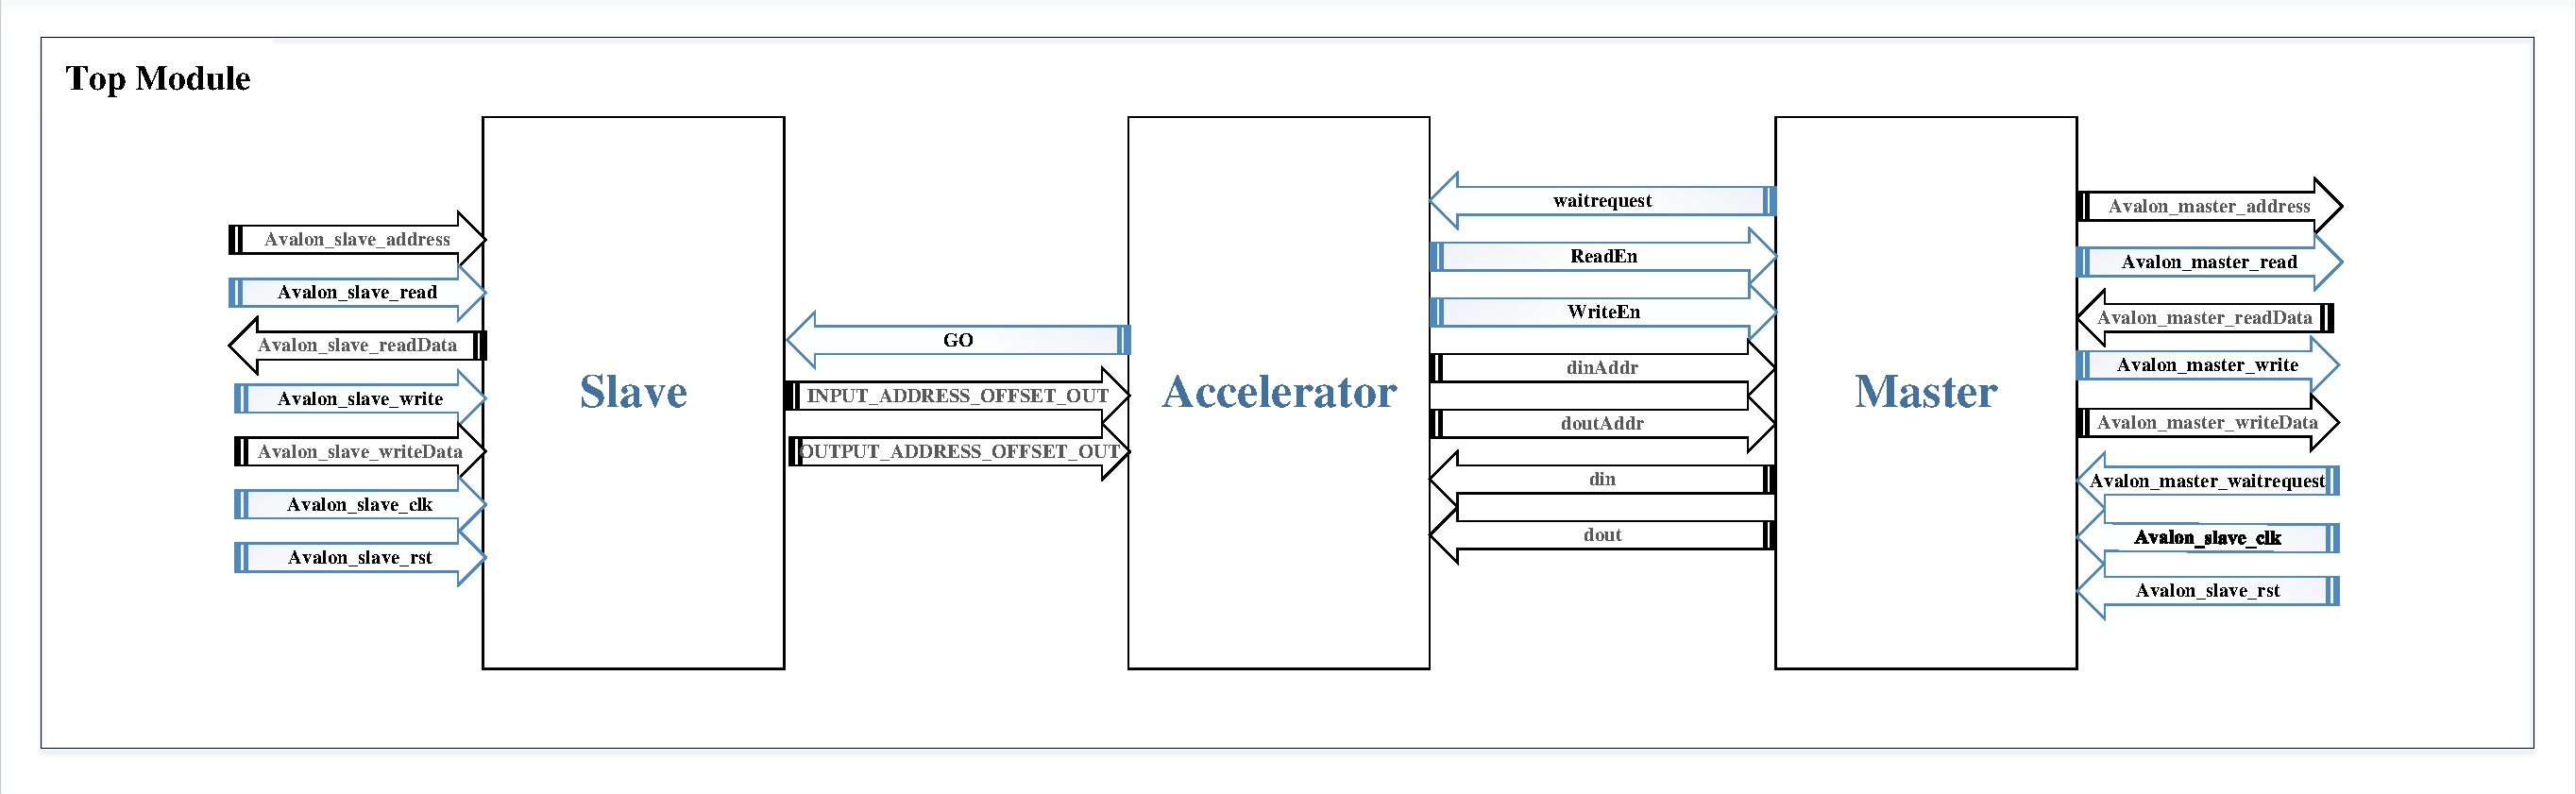
\includegraphics[width=0.4\textwidth]{Master_Slave_Diagram.pdf}
  \caption{Figure 1}
  \label{fig:visio-diagram}
\end{figure}

% \begin{description}
% \item[First] This is the first item
% \item[Last] This is the last item
% \end{description}

% \lipsum[9] % Dummy text

\section*{\small{System Design in Qsys}}

% \lipsum[8] % Dummy text

After designing the accelerator in VHDL, it is necessary to transfer this 
module into the Qsys environment for integration with the system. In Qsys, 
it is important to ensure that signals are properly configured as either Signed or Unsigned, 
depending on their use. Small adjustments are required to ensure proper synthesis of the 
designed system.

\section*{\small{Building the System}}

% \lipsum[8] % Dummy text

The system must be built and tested using the Nios II Software Build Tools for Eclipse. 
In this step, we generate the BSP (Board Support Package) and write a program to interact 
with the accelerator. This program reads image data from memory, sends it to the accelerator 
for processing, and retrieves the processed data.

\section*{\small{Conclusion}}

% \lipsum[8] % Dummy text

The designed accelerator was successfully integrated into the system and was able to process image 
data using the edge detection filter. The results from the testbench demonstrate that the system 
operates as expected, with the processed image data correctly written back to memory after filtering. 
Further improvements could include optimizing the accelerator for speed and adding additional filters.

%----------------------------------------------------------------------------------------
%	REFERENCE LIST
%----------------------------------------------------------------------------------------

\begin{thebibliography}{99} % Bibliography - this is intentionally simple in this template

  \bibitem[Alipour Fraydani, 2024]{AlipourFraydani:2024}
  Alipour Fraydani, A. (2024).
  \newblock Homework on Methodology and automatic design algorithms of digital systems, University of Tehran.
  \newblock {\em Unpublished Manuscript}, Department of Electrical Engineering, University of Tehran.
  
\end{thebibliography}

%----------------------------------------------------------------------------------------

\end{document}